%!TEX program = xelatex
% 完整编译: xelatex -> bibtex -> xelatex -> xelatex
\documentclass[lang=cn,11pt,a4paper]{elegantpaper}

\usepackage{calc}
\usepackage{times}
\usepackage{float}

\usepackage{pdfpages}

\usepackage{amssymb} % \Box
%\usepackage{algorithm}  
%\usepackage{algorithmicx}  
\usepackage{algpseudocode}
\usepackage{amsmath}
\usepackage[linesnumbered,ruled,lined]{algorithm2e}
\usepackage{graphicx}
\usepackage{listings}
\usepackage{color}
\usepackage{colortbl}
\usepackage{longtable}
\SetArgSty{textnormal} % non-italics in if-clause of algorithm

\usepackage{hyperref}
\usepackage{titlesec}
\titleformat{\section}{\centering\Huge\bfseries}{\thesection}{1em}{}
\titleformat{\subsection}{\LARGE\bfseries}{\thesubsection}{1em}{}

\title{计算机系统综合实验手册}
% \author{欧先飞 \\ ouxianfei@smail.nju.edu.cn}

%\institute{\href{https://elegantlatex.org/}{Elegant\LaTeX{} 项目组}}

%\newcommand{\blankbox}{\boxed{\textcolor[rgb]{1,1,1}{*}}}
\newcommand{\blankbox}{\Large{\qedsymbol}}

%\version{0.08}
%\date{\zhtoday}

\begin{document}

\maketitle

\tableofcontents

\newpage

\section{基本工具链}

本节所涉及的内容,是为开展计算机系统综合实验的必要基础,请务必完全熟练掌握。

\subsection{git基本用法}

git的教程有很多,这里不详细叙述git的各种基本运作机制,仅从样例出发,讲解必要掌握的命令。

首先是最基本的clone项目:
\begin{lstlisting}
git clone https://github.com/your/repo
git clone git@github.com:your/repo # 需将你的公钥上传到github上
\end{lstlisting}

上传公钥:
\begin{lstlisting}[language=bash]
# 先生成密钥
~bash> cd ~/.ssh && ls -al
. ..
~bash> ssh-keygen -t rsa -C "you@email.cn"
Generating public/private rsa key pair.
Enter file in which to save the key (/home/you/.ssh/id_rsa):
Enter passphrase (empty for no passphrase): 
Enter same passphrase again: 
Your identification has been saved in /home/you/.ssh/id_rsa.
Your public key has been saved in /home/you/.ssh/id_rsa.pub.
The key fingerprint is:
SHA256:ORKaY5n3N4G0P4guAbT0UFNZNorA3mqSL0S0xPWo/+U you@email.cn
The key's randomart image is:
+---[RSA 2048]----+
|..ooo..o+        |
| +=.oo.o .       |
|o+.*..o .        |
| o= o= o +       |
|.o oB o S .      |
|o.+..o + + .     |
|.+ . ...o =      |
|. . o.o  . o     |
| .   o.E         |
+----[SHA256]-----+
~bash> ls # 现在可以看到id_rsa.pub文件
id_rsa  id_rsa.pub
~bash>
\end{lstlisting}
进入github的settings -> SSH and GPG keys -> New SSH Key,然后将id\_rsa.pub的内容拷贝进去即可。

除了克隆项目,还有如下必要用法:
\begin{lstlisting}
git push # 推送
git pull # 拉取
\end{lstlisting}

对远程仓库的管理:
\begin{lstlisting}
git remote -v # 查看远程仓库的情况

# 绑定一个远程仓库git@github.com:new/repo并将其命名为origin
git remote add origin git@github.com:old/repo

# 将仓库名origin所绑定的远程仓库地址更改为git @github.com:new/repo
git remote set-url origin git @github.com:new/repo

# 将本地的local分支推送到远程的remote分支
git push origin local:remote

# 将本地的local分支强制推送到远程的remote分支,如有冲突,覆盖掉远程的项目
git push -f origin local:remote

# 加上-u可以设置缺省推送参数,即后续只需git push即可
git push -u origin local:remote
\end{lstlisting}

对本地项目的管理:
\begin{lstlisting}
# 保存当前目录所有更改并提交到本地仓库
git add . -A && git commit -m 'message'

# 追加提交
git commit --amend -m 'new message'

# 用352cdeca2caa8a309d2所保存的文件覆盖掉当前目录
git checkout 352cdeca2caa8a309d2 .

# 查看352cdeca2caa8a309d2这一提交时README.md的内容
git show 352cdeca2caa8a309d2:./README.md
git show 352cdeca2caa8a309d2:./README.md | vim -

git log # 查看本地项目的变更历史
git reflog # 查看本地项目的完整变更历史,包括所有reset都记录在内
git reset --hard 352cdeca2caa8a309d2 # 回退到352cdeca2caa8a309d2,同时回退目录下的文件
git reset --soft 352cdeca2caa8a309d2 # 只回退git记录,不回退文件内容
\end{lstlisting}

\subsection{Makefile}\label{Makefile}

写在前面,对于过于复杂的Makefile,可以使用\lstinline!make -nB target!来查看生成\lstinline!target!时会执行到的指令,这对于了解一个Makefile究竟干了什么非常有用。除此以外Makefile里面可以通过\lstinline!$(info "xxx")!来打印字符串,这个对于调试Makefile非常有用。

\subsubsection{规则依赖}

一个简单的例子:
\begin{lstlisting}
a.o: a.c
  g++ a.c -o a.o

b.o: b.c
  g++ b.c -o b.o

binary: a.o b.o
  echo + binary
\end{lstlisting}

将上述内容写入到你当前目录的Makefile文件中,并保证\lstinline!a.c!和\lstinline!b.c!文件存在,然后在命令行里敲\lstinline!make binary!,这条语句的意思是制造\lstinline!binary!这个目标,make会读特定名称的文件来获取制造这个目标的规则(Makefile是make内置的一个特定名称)。make读取你的Makefile后会发现binary依赖于\lstinline!a.o!和\lstinline!b.o!,并进而计算得出\lstinline!a.o!依赖于\lstinline!a.c!,\lstinline!b.o!依赖于\lstinline!b.c!,最后按照你给定的生成规则\lstinline!g++ a.c -o a.o!和\lstinline!g++ b.c -o b.o!去生成相应的\lstinline!a.o!和\lstinline!b.o!。

敲完\lstinline!make binary!之后,你binary并没有生成,因为你还没有为binary添加生成规则,所以如果你再敲一遍\lstinline!make binary!,相应的\lstinline!echo + binary!语句会被再执行一遍。

我们稍微改一下,让他变成下面这样:
\begin{lstlisting}
a.o: a.c
  g++ a.c -o a.o

b.o: b.c
  g++ b.c -o b.o

binary: a.o b.o
  cat a.o b.o > binary
\end{lstlisting}

这个时候如果你在敲\lstinline!make binary!,生成规则会将\lstinline!a.o!与\lstinline!b.o!拼接成binary文件,由于binary文件是最新生成的,它的时间戳大于\lstinline!a.o!和\lstinline!b.o!的时间戳,所以再下一次你敲\lstinline!make binary!的时候,make会输出\lstinline!'binary' is up to date!。

一般而言,我们并不希望我们所生成的中间文件和源码文件共用一个目录,假设我们希望将目录结构调整成这样:
\begin{lstlisting}
+---src
|   +--- a.c
|   +--- b.c
|
+---build
    +--- a.o
    +--- b.o
    +--- binary
\end{lstlisting}

为了达成这个目的,我们需要对Makefile做一些微调:
\begin{lstlisting}
build/a.o: src/a.c
  mkdir -p build
  g++ src/a.c -o build/a.o

build/b.o: b.c
  mkdir -p build
  g++ src/b.c -o build/b.o

build/binary: build/a.o build/b.o
  cat build/a.o build/b.o > build/binary
\end{lstlisting}

相应的,基于这个Makefile来生成binary,我们需要执行\lstinline!make build/binary!,这条命令会按照你的规则去生成\lstinline!build/a.o!和\lstinline!build/b.o!两个文件,然后拼接成\lstinline!build/binary!这个文件。

这个时候,你可能发现,make的时候连目录一起写进去太撒刁了,所以这个Makefile可以进一步改进:

\begin{lstlisting}
.PHONY: binary

binary: build/binary

build/a.o: src/a.c
  mkdir -p build
  g++ src/a.c -o build/a.o

build/b.o: b.c
  mkdir -p build
  g++ src/b.c -o build/b.o

build/binary: build/a.o build/b.o
  cat build/a.o build/b.o > build/binary
\end{lstlisting}

\lstinline!.PHONY!的作用是定义一个伪目标,什么是伪目标,直观的讲就是,这个目标在磁盘上不存在。之前Makefile里面的\lstinline!a.o!、\lstinline!build/binary!、\lstinline!build/a.o!这些目标在磁盘上是会对应到一个实际存在的文件的,而伪目标不需要满足这个要求,同时相应的,make也不会去检查伪目标的时间戳,而是直接调用他的生成规则,比如:

\begin{lstlisting}

.PHONY: hello

hello:
  touch hello
  echo hello world
\end{lstlisting}

在这个makefile中,无论你敲几次\lstinline!make hello!,\lstinline!touch hello!和\lstinline!echo hello world!这两条生成规则都会被执行。

\subsubsection{通用匹配\%和生成规则简化}

在上文提到的Makefile中,你会发现在编写a.o和b.o的生成规则的时候,你需要把\lstinline!build/!和\lstinline!a.o!这样的多余的东西再写一遍,这个信息明明已经包含在依赖目标和生成目标里了,为了简化规则的编写,makefile定义了一系列的简写符号,用这些符号我们可以将Makefile简化成:

\begin{lstlisting}
.PHONY: binary

binary: build/binary

build/a.o: src/a.c
  mkdir -p $(@D)
  g++ $^ -o $@

build/b.o: b.c
  mkdir -p $(@D)
  g++ $^ -o $@

build/binary: build/a.o build/b.o
  cat $^ > $@
\end{lstlisting}

其中\lstinline!$^!出现在生成规则中表示所有被依赖的目标(示例中\lstinline!$^!会被替换成\lstinline!build/a.o build/b.o!),\lstinline!$@!表示生成的目标(示例中上下两条生成规则里的\lstinline!$@!分别会被替换成\lstinline!build/a.o!和\lstinline!build/b.o!),\lstinline!$(@D)!则是表示生成目标所在的目录,也就是\lstinline!build/!,所以上面的Makefile其实与之前的Makefile完全等价。

\begin{table}[htbp]
\centering
\begin{tabular}{|c|c|}
\hline
符号&含义 \\\hline
\lstinline|$(@D)| & 当前规则目标所在目录 \\\hline
\lstinline|$@| & 当前规则目标 \\\hline
\lstinline|$<| & 当前规则依赖项的第一个 \\\hline
\lstinline|$^| & 当前规则的所有依赖项 \\\hline
\end{tabular}
\caption{规则匹配中常见符号}
\end{table}

到这里,你会发现一件更撒刁的事,那就是\lstinline!mkdir -p $(@D)!和\lstinline!g++ $^ -o $@!这两条语句你在两个目标的生成规则中写了两遍,为了解决这样的问题,Makefile又提供了通配符机制,利用通配符,我们可以将Makefile进一步改写成:

\begin{lstlisting}
.PHONY: binary

binary: build/binary

build/%.o: src/%.c
  mkdir -p $(@D)
  g++ $^ -o $@

build/binary: build/a.o build/b.o
  cat $^ > $@
\end{lstlisting}

在这个Makefile上,如果我们敲\lstinline!make binary!,make会去查找\lstinline!build/binary!所依赖的\lstinline!build/a.o!和\lstinline!build/b.o!的生成规则,当然make是找不到的,因为我们并没有明确的写这样的规则。但是make会进一步发现,它只要把\lstinline!build/%.o!中的\lstinline!%!这个字符替换成\lstinline!a!,他就能匹配上\lstinline!build/%.o: src/%.c!这条规则,于是它就把这条规则里面所有的\lstinline!%!都替换成了\lstinline!a!,便得到了\lstinline!build/a.o!的生成规则,同理它也能获得\lstinline!build/b.o!的生成规则。

\subsubsection{变量和函数的使用}

在上面的Makefile里面,我们还有着这样一个问题,就是如果我们不知道src下面究竟有多少\lstinline!.c!文件,但是我们依旧希望Makefile能工作应该怎么办。举个简单的场景,你的项目正在如火如荼的发展中,每天都可能添加若干个\lstinline!.c!文件或重命名若干个\lstinline!.c!文件,如果你每次都要手动更新Makefile,未免太过撒刁了,为了解决这个问题,Makefile提供了函数机制。

回顾我们的需求,我们其实需要的是make能自动找到src下所有的.c文件,并将其重命名为build下的.o文件,最后放到\lstinline!build/binary!的依赖目标中去:

\begin{lstlisting}
.PHONY: binary

binary: build/binary

build/%.o: src/%.c
  mkdir -p $(@D)
  g++ $^ -o $@

build/binary: $(patsubst src/%.c,build/%.o,$(shell find src/ -name "*.c"))
  cat $^ > $@
\end{lstlisting}

新的Makefile中\lstinline!build/binary!所依赖的目标已经被替换成了\lstinline!$(patsubst src/%.c,build/%.o,$(shell find src/ -name "\*.c"))!,我们分开来讲这条语句,首先是\lstinline!$(shell find src/ -name "\*.c")!,这条语句会调用你终端中的\lstinline!find!命令,查找\lstinline!src!目录下所有的\lstinline!.c!文件,并将其替换成查找的结果,也就是说这条语句执行完毕之后原语句会变成\lstinline!$(patsubst src/%.c,build/%.o,src/a.c src/b.c)!,\lstinline!patsubst!是make的一个内置函数,它的作用是根据你指定的初始特征和结果特征,对你的输入进入转化,对应到这条语句,你给它的初始特征是\lstinline!src/%.c!,结果特征是\lstinline!build/%.o!,输入是\lstinline!src/a.c src/b.c!,对于输入中的每一项,如\lstinline!src/a.c!,\lstinline!patsubst!函数会发现将\lstinline!%!换成\lstinline!a!就能匹配上,然后他讲结果特征中的\lstinline!%!也换成\lstinline!a!,并将结果替换掉\lstinline!src/a.c!,也就是说,\lstinline!src/a.c!会被替换成\lstinline!build/a.o!,同理\lstinline!src/b.c!也会被替换成\lstinline!build/b.o!。

上述Makefile看着非常蛋疼,因为我们写了一个超长的语句,有没有一种机制,像编程语言一样,通过定义一些中间变量来拆分超长表达式呢?答案当然是有的,所以上面的Makefile又可以改成下面这样:

\begin{lstlisting}
.PHONY: binary

SRC_DIR := src/
SRCS    := $(shell find $(SRC_DIR) -name "*.o")
OBJ_DIR := build/
OBJS    := $(patsubst src/%.c,build/%.o,$(SRCS))

binary: $(OBJ_DIR)binary

$(OBJ_DIR)%.o: $(SRC_DIR)%.c
  mkdir -p $(@D)
  g++ $^ -o $@

$(OBJ_DIR)binary: $(OBJS)
  cat $^ > $@
\end{lstlisting}

上面的赋值使用了\lstinline!:=!,你暂时不需要知道为什么是\lstinline!:=!而不是\lstinline!=!,如果你真的想了解,在docs目录下的Makefile.pdf可以给你答案,同时如果哪天你需要什么其它的功能,你也可以通过查阅\lstinline!Makefile.pdf!来看看是否有相应的函数。

\begin{table}[htbp]
\centering
\begin{tabular}{|c|c|}
\hline
函数&含义(具体用法请查询\href{run:../manuals/Makefile.pdf}{手册}) \\\hline
\lstinline|$(shell xxx)| & 执行shell命令,并将结果替换到当前位置 \\\hline
\lstinline|$(dir ...)| & 获取目录 \\\hline
\lstinline|$(notdir ...)| & 获取文件名 \\\hline
\lstinline|$(realpath ...)| & 将相对路径转化为绝对路径 \\\hline
\lstinline|$(foreach v, ..., ...)| & 遍历 \\\hline
\lstinline|$(eval ...)| & 根据输入的字符串生成新规则 \\\hline
\lstinline|$(subst , , ...)| & 子串替换 \\\hline
\lstinline|$(patsubst , ..., ...)| & 基于特征的子串替换 \\\hline
\end{tabular}
\caption{Makefile常用函数}
\end{table}

\subsubsection{宏的使用与自动规则生成}

假如你想把你的Makefile包装成一个功能库,其他人只要include你的Makefile就能获得上述所有的功能,那么你需要怎么做呢?一个简单的答案就是宏。

待续。。。

\subsection{verilator}\label{verilator}
verilator可以将我们的verilog代码使用C++模拟,从而使用C++语言可以编写测试程序。verilator将我们的verilog代码编译成一个类,我们只需要在我们的测试的.c文件中include其生成的头文件即可。

\subsubsection{前置说明}
verilator的用法,在样例工程中均有体现,建议从样例工程入手,辅之以手册博客,样例项目参见\href{run:../examples/1.Makefile-chisel-sample}{examples/1.Makefile-chisel-sample}。

\subsubsection{使用makefile组织verilator}
从样例项目出发,组织一个工程的makefile,首先得知道这个工程的编译流程以及需要的项目目录的组织(将源代码和生成的代码放置在不同的文件夹中),其次将编译过程中的重要的中间文件确定出来,将其固定命名,这样可以使得makefile的流程更加简单易维护,然后按照这些中间文件的编译顺序来编写makefile,确定依赖,使用知道的编译命令逐步编译.

\subsubsection{Makefile代码解析}
\begin{lstlisting}
.PHONY: xxx
\end{lstlisting}
.PHONY定义的伪目标的作用是能够使得makefile在每次make的时候将这个目标下的指令重新做一遍,因为当依赖没有改变时,makefile会默认这个过程不需要再执行一次,但有时候我们需要这个目标作为一个常用的调用执行,这样可以将它定义为伪目标

\begin{lstlisting}
SCALA_FILES := $(shell find $(SCALA_DIR) -name "*.scala")
\end{lstlisting}
这个指令的作用是将**SCALA\_DIR**目录下寻找所有的**scala**后缀的文件.
\begin{lstlisting}
$(EMU_TOP_V): $(SCALA_FILES)
	@mkdir -p $(@D)
	@sbt "run MainDriver -tn $(EMU_TOP_MODULE) -td $(@D) --output-file $@"
\end{lstlisting}
这一段是将SCALA文件使用sbt编译成对应的.v文件,前面的@标记会使得这条命令不出现在命令行中.
\begin{lstlisting}
$(EMU_MK): $(EMU_TOP_V) $(EMU_CXXFILES)
	@verilator --cc --exe --top-module $(EMU_TOP_MODULE) \
	  -o $(notdir $(EMU_BIN)) -Mdir $(@D) \
	  --prefix $(basename $(notdir $(EMU_MK))) $^ 
\end{lstlisting}
这一段将之前生成的.v文件和我们编写的cpp文件一起编译成verilator的bin文件, --cc是说明使用C++, --exe是说明和cpp一起编译生成一个可执行工程, --top-module是用于指定出需要编译的顶层模块. -o指定最后生成的可执行文件名, -Mdir指明verilator生成文件所在目录, --prefix指明使用的.mk文件.

\begin{lstlisting}
$(EMU_BIN): $(EMU_MK) $(EMU_CXXFILES)
	@cd $(@D) && make -s -f $(notdir $<)
\end{lstlisting}
这一段将verilator工具生成的代码使用其规则来make出最后的可执行文件.

\subsubsection{emu/main.cpp解释}
\begin{lstlisting}
#include "emu.h"
#include <memory>
#include <iostream>
#include <verilated.h>

int main(int argc, char **argv) {

/*emu是verilator工具为我们的verilog代码生成的一个类。*/
  auto dut = std::make_shared<emu>();	

/*dut->reset表示的是我们的verilog代码中的一个输入信号。*/

  dut->reset = 0;					
  for (int i = 0; i < 10; i++) {
    dut->io_in_valid = 1;
    dut->io_in_bits_op = i;
    dut->io_in_bits_a = 123;
    dut->io_in_bits_b = 456;

/*以下4句代码表示了一个周期的变化,clock置0再置1,即为一个周期的变化*/

    dut->clock = 0;							
    dut->eval();								//更新类中各个信号的信息

    dut->clock = 1;
    dut->eval();

/*打印出电路模拟的时候的某个信号的信息,可以写相关代码自动判断信号是否出错*/
	printf ("RECEIVE: %d\n", dut->io_out_bits_c);
  }
  return 0;
}
\end{lstlisting}

\subsection{Chisel}
chisel是由伯克利开发的一门硬件构建语言,嵌入在scala编程语言中。相比verilog,chisel有抽象的数据类型和接口,层次化+面向对象+功能化构造,可以很简单地实现工程的高度参数化。可以编译生成出verilog语言,相当于软件设计语言中的高级语言。

\subsubsection{chisel安装}
使用chisel语言需要安装sbt
官方网站:\url{https://www.scala-sbt.org/1.0/docs/Installing-sbt-on-Linux.html}

\begin{lstlisting}
$ echo "deb https://dl.bintray.com/sbt/debian /" | sudo tee -a /etc/apt/sources.list.d/sbt.list
$ sudo apt-key adv --keyserver hkps://keyserver.ubuntu.com:443 --recv 2EE0EA64E40A89B84B2DF73499E82A75642AC823
$ sudo apt-get update
$ sudo apt-get install sbt
\end{lstlisting}

\subsubsection{用chisel编写硬件}
\begin{lstlisting}
git clone https://github.com/addrices/chisel-template.git
\end{lstlisting}
这是使用chisel语言的一个简单的例子,即本项目下 examples/Makefile-chisel-sample,可以直接从上面的仓库获得。
我们简单分析一下这个项目中的各个文件的作用:

这个简单的项目是使用chisel编写硬件并且使用verilator来进行测试。Makefile文件中命令的详细解释放置在verilator.md中。

\begin{lstlisting}
import chisel3._
import chisel3.util._
import chisel3.iotesters.{ChiselFlatSpec, Driver, PeekPokeTester}

/*类似于c语言中的函数,可以在电路重复的地方复用*/
object GTimer {
  def apply(): UInt = {
    val (t, c) = Counter(true.B, 0x7fffffff)
    t
  }
}

/*类似于c语言中的结构体,将相关的信号线打包成一个结构体,其中的Output表示输出(Input是输入)*/
class ALU_IN extends Bundle {
  val op = Output(UInt(4.W))
  val b = Output(UInt(32.W))
  val a = Output(UInt(32.W))
}

class ALU_OUT extends Bundle {
  val c = Output(UInt(32.W))
}

class ALU extends Module {
    //表示当前ALU模块的输入输出的信号定义
  val io = IO(new Bundle {
   //这里的Flipped表示的是该结构体中所有Input信号变成Output信号,Output信号变成Input信号
    val in = Flipped(ValidIO(new ALU_IN))            
    val out = ValidIO(new ALU_OUT)
  })

  io.in := DontCare

  /* in is valid at the next cycle of valid io.in */
  val in_valid = RegNext(io.in.valid, init=false.B)
  val in = RegEnable(enable=io.in.valid, next=io.in.bits,
    init=0.U.asTypeOf(io.in.bits))

  val neg_b = Mux(in.op(3) === 0.U, in.b, ~in.b + 1.U)
  val sr = Mux(in.op(3) === 0.U,
    in.a >> (in.b(4, 0)),
    (in.a.asSInt >> (in.b(4, 0))).asUInt)

  io.out.valid := in_valid
  io.out.bits.c := Mux1H(Seq(
    (in.op(2, 0) === 0.U) -> (in.a + neg_b),
    (in.op(2, 0) === 1.U) -> (in.a << (in.b(4, 0))),
    (in.op(2, 0) === 2.U) -> (in.a.asSInt < in.b.asSInt).asUInt,
    (in.op(2, 0) === 3.U) -> (in.a < in.b).asUInt,
    (in.op(2, 0) === 4.U) -> (in.a ^ in.b),
    (in.op(2, 0) === 5.U) -> (sr),
    (in.op(2, 0) === 6.U) -> (in.a | in.b),
    (in.op(2, 0) === 7.U) -> (in.a & in.b )
  ))

  when (in_valid) {
    printf("CLOCK: %x, op: %x, a: %x, b: %x; c: %x\n",
      GTimer(), in.op, in.a, in.b, io.out.bits.c)
  }
}

//这个函数是为chisel代码生成verilog代码使用的。指定最后生成的顶层模块即可。
object MainDriver extends ChiselFlatSpec {
  def main(args: Array[String]): Unit = {
    chisel3.Driver.execute(args, () => new ALU)
  }
}
\end{lstlisting}
在根目录下输入
\begin{lstlisting}
$ sbt
... # 一堆sbt的输出
sbt $ run MainDriver -tn [顶层模块] -td [源文件目录] --output-file [目的地址文件]
\end{lstlisting}
即可获得对应的.v文件
\subsubsection{相关网站}
伯克利的Chisel教程: \url{https://github.com/ucb-bar/chisel-tutorial}

chisel api查询: \url{https://www.chisel-lang.org/api/latest/index.html}

\subsection{minicom的使用方法}

minicom是一款终端串口连接软件,并且minicom自己有一套脚本语法,便于在不定延迟的串口上传送指令

\subsubsection{基本的使用}
将开发板上的uart接口和电脑的usb接口相连接,此时在你的ubuntu的/dev目录下会多出一个ttyUSB1文件,这个文件就是用于连接串口的钥匙
\begin{itemize}
\item 连接串口: \lstinline!sudo minicom -D /dev/ttyUSB1 -b 115200!
\begin{itemize}
\item \lstinline!-D /dev/ttyUSB1!的含义显而易见,这里的设备文件有时候是\lstinline!/dev/ttyUSB0!,具体看实际情况
\item \lstinline!-b 115200!用于指定串口的波特率,可以理解为传数据的频率,115200就是每秒传115200个比特 (\textcolor{red}{注意:上板设置的波特率和minicom设置的波特率一定要一样,不然会乱码})
\end{itemize}
\item 开启escape控制码: \lstinline!minicom -c on ...!
\begin{itemize}
\item 一般情形你在终端里\lstinline!printf "\e[32mHelloWorld\e[0m"!是会出现彩色文字的(因为这里使用了控制码\lstinline!\e[32m!),彩色文字便于在调试的时候快速定位关键信息,但是minicom从串口接受数据并显示的时候会把彩色(escape控制码)给过滤掉,你可以通过\lstinline!-c on!开启彩色显示
\end{itemize}
\end{itemize}

\subsubsection{minicom脚本}
一个你们开始上板时会频繁出现的需求,那就是自动化启动加载过程,因为从上板开始,到你们加载cpu完毕,你们需要在串口里敲很多命令,而自动化可以给你们省下很多时间:

一个简单的例子,如果你需要启动u-boot,然后从网口加载程序到cpu上,经常会敲的指令:
\begin{lstlisting}
UBOOT> set serverip 192.168.1.104
UBOOT> set ipaddr 192.168.1.107
UBOOT> set gateway 192.168.1.104
UBOOT> tftpboot 0x82000000 nanos-pal
UBOOT> bootelf -p 0x82000000
\end{lstlisting}
这几条命令还有一个限制,那就是每次敲的时候都必须等待相应的提示符出现之后才能敲命令,过早的敲会被无效掉,而将这一过程写成脚本就是:
\begin{lstlisting}
START:

gosub WAIT_PROMPT
send "set serverip 192.168.1.104"

gosub WAIT_PROMPT
send "set ipaddr 192.168.1.107"

gosub WAIT_PROMPT
send "set gateway 192.168.1.104"

gosub WAIT_PROMPT
send "tftpboot 0x82000000 nanos-pal"

gosub WAIT_PROMPT
send "bootelf -p 0x82000000"

exit

WAIT_PROMPT:
expect {
  "UBOOT> " break
  goto FAIL
}
return

FAIL:
\end{lstlisting}
然后下次你再连接串口的时候,使用指定这个脚本就行了(假设上述内容写入了minicom.script这个文件): \lstinline!sudo minicom -D /dev/ttyUSB1 -b 115200 -c on -S minicom.script!

\subsubsection{minicom的日志记录功能}
有的时候你可以需要让minicom把所有的内容都记下来,这个时候你加上一个\lstinline!-C xx.log!选项就行了,这个选项会将所有内容追加到\lstinline!xx.log!这个文件末尾。

\subsection{ILA的使用方法}

在最坏的情况下,你的cpu模拟可以跑,仿真可以跑,唯独上板不能跑,这个时候你便需要在上板的时候采样一些信号,来帮助你判断上板运行的状态以及进一步的调试。

有2中方法可以设置ILA,一种是在.v文件中生成,第二种是使用block design设置。
\subsubsection{代码设置}

在你需要采样的信号的定义前加上 
\begin{lstlisting}
(*mark_debug = "true"*)
\end{lstlisting}
如图所示:
\begin{figure}[H]
\centering
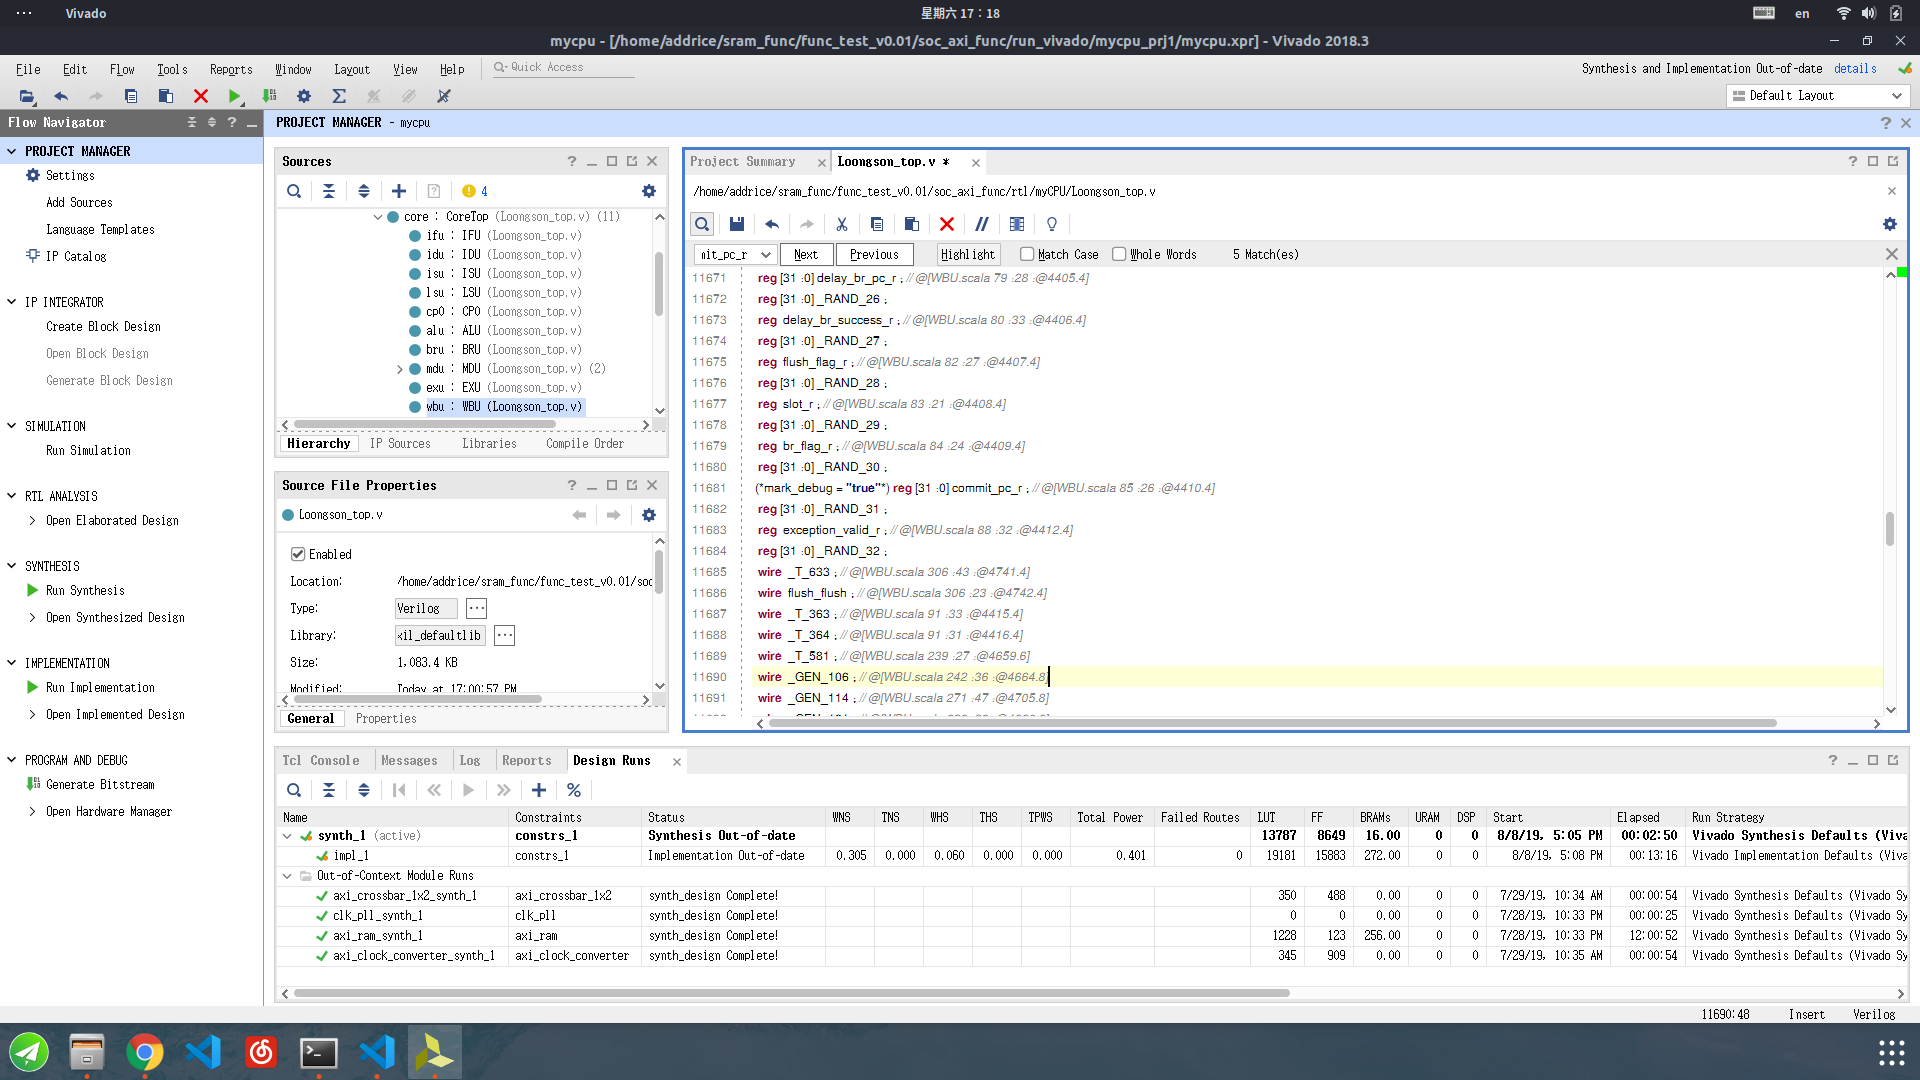
\includegraphics[width=\linewidth]{image/mark_debug_1.png}
\end{figure}

然后综合(Run synthesis),完成后open Synthesized Design,点击Set up Debug,如图所示
\begin{figure}[H]
\centering
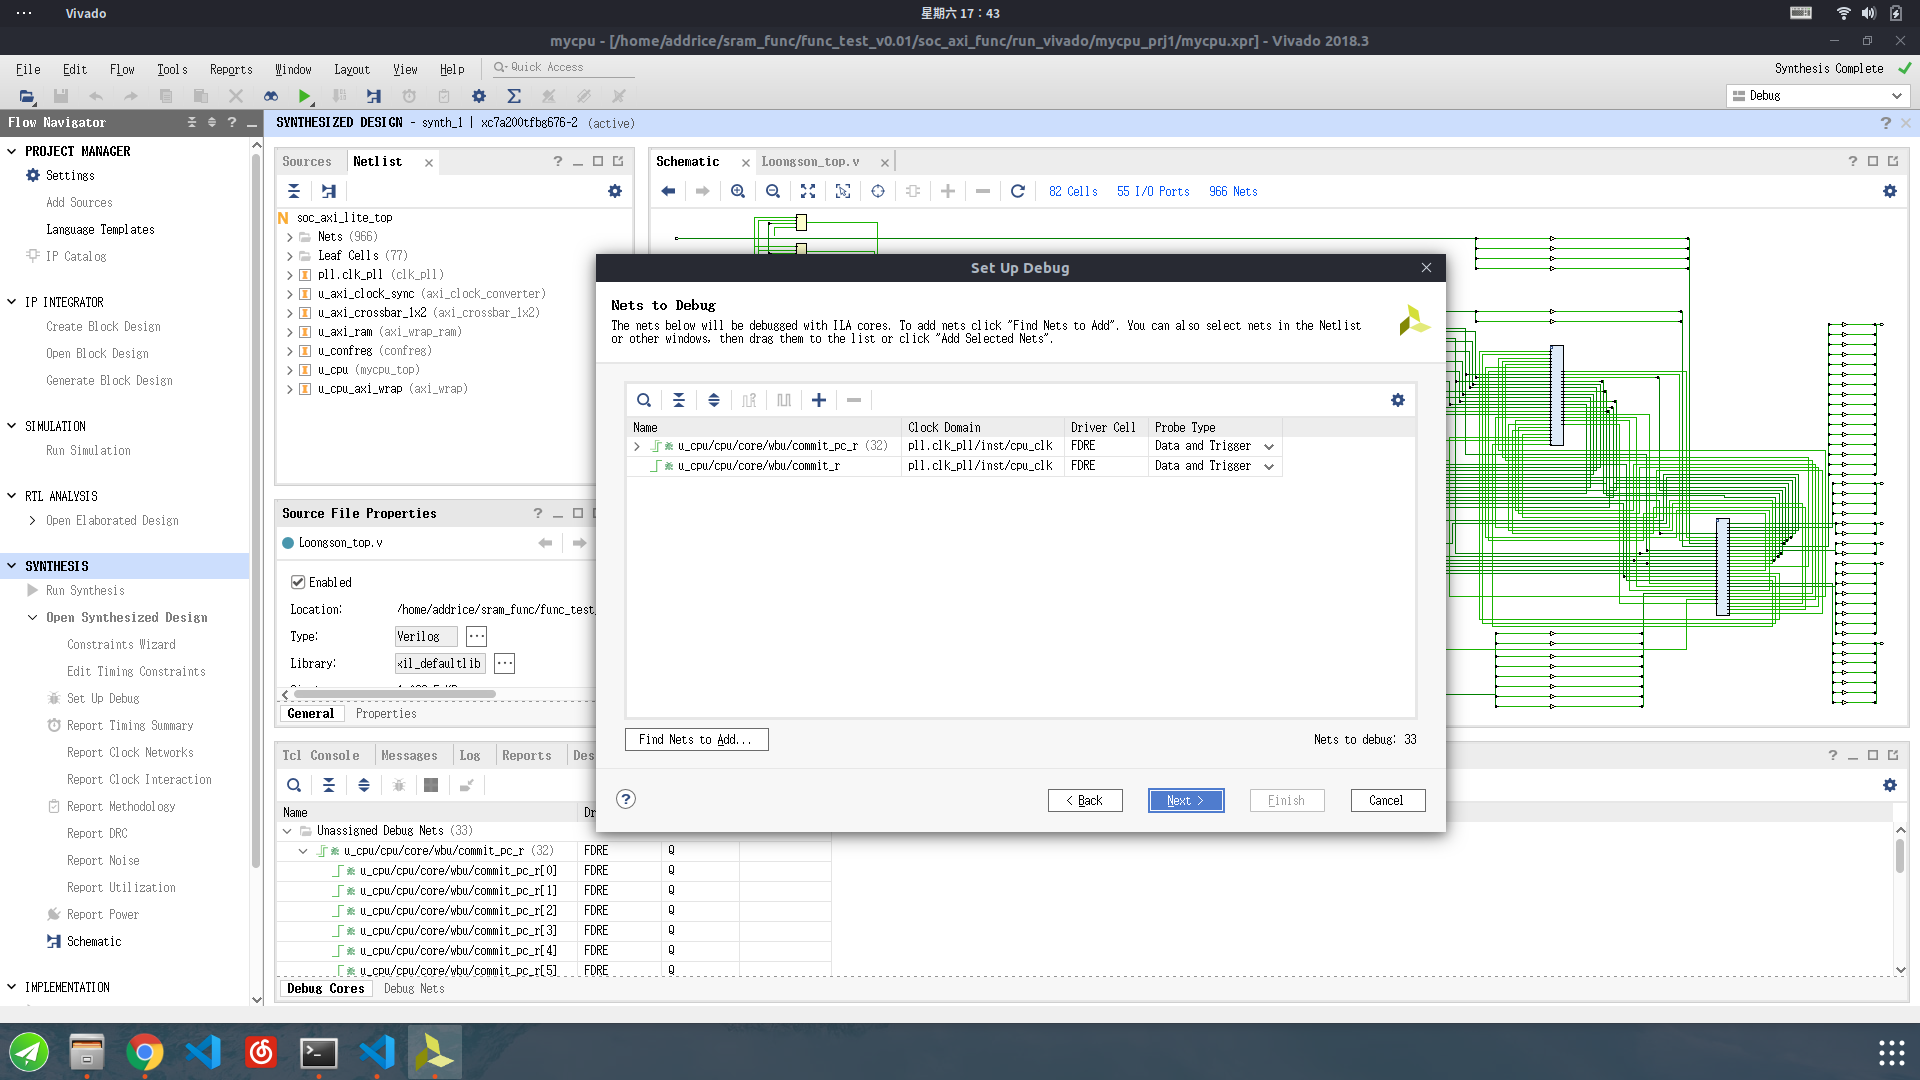
\includegraphics[width=\linewidth]{image/mark_debug_2.png}
\end{figure}
设置过的mark\_debug的信号会显示在其中,点击next,勾选Captrue control和Advanced trigger,如图所示

\begin{figure}[H]
\centering
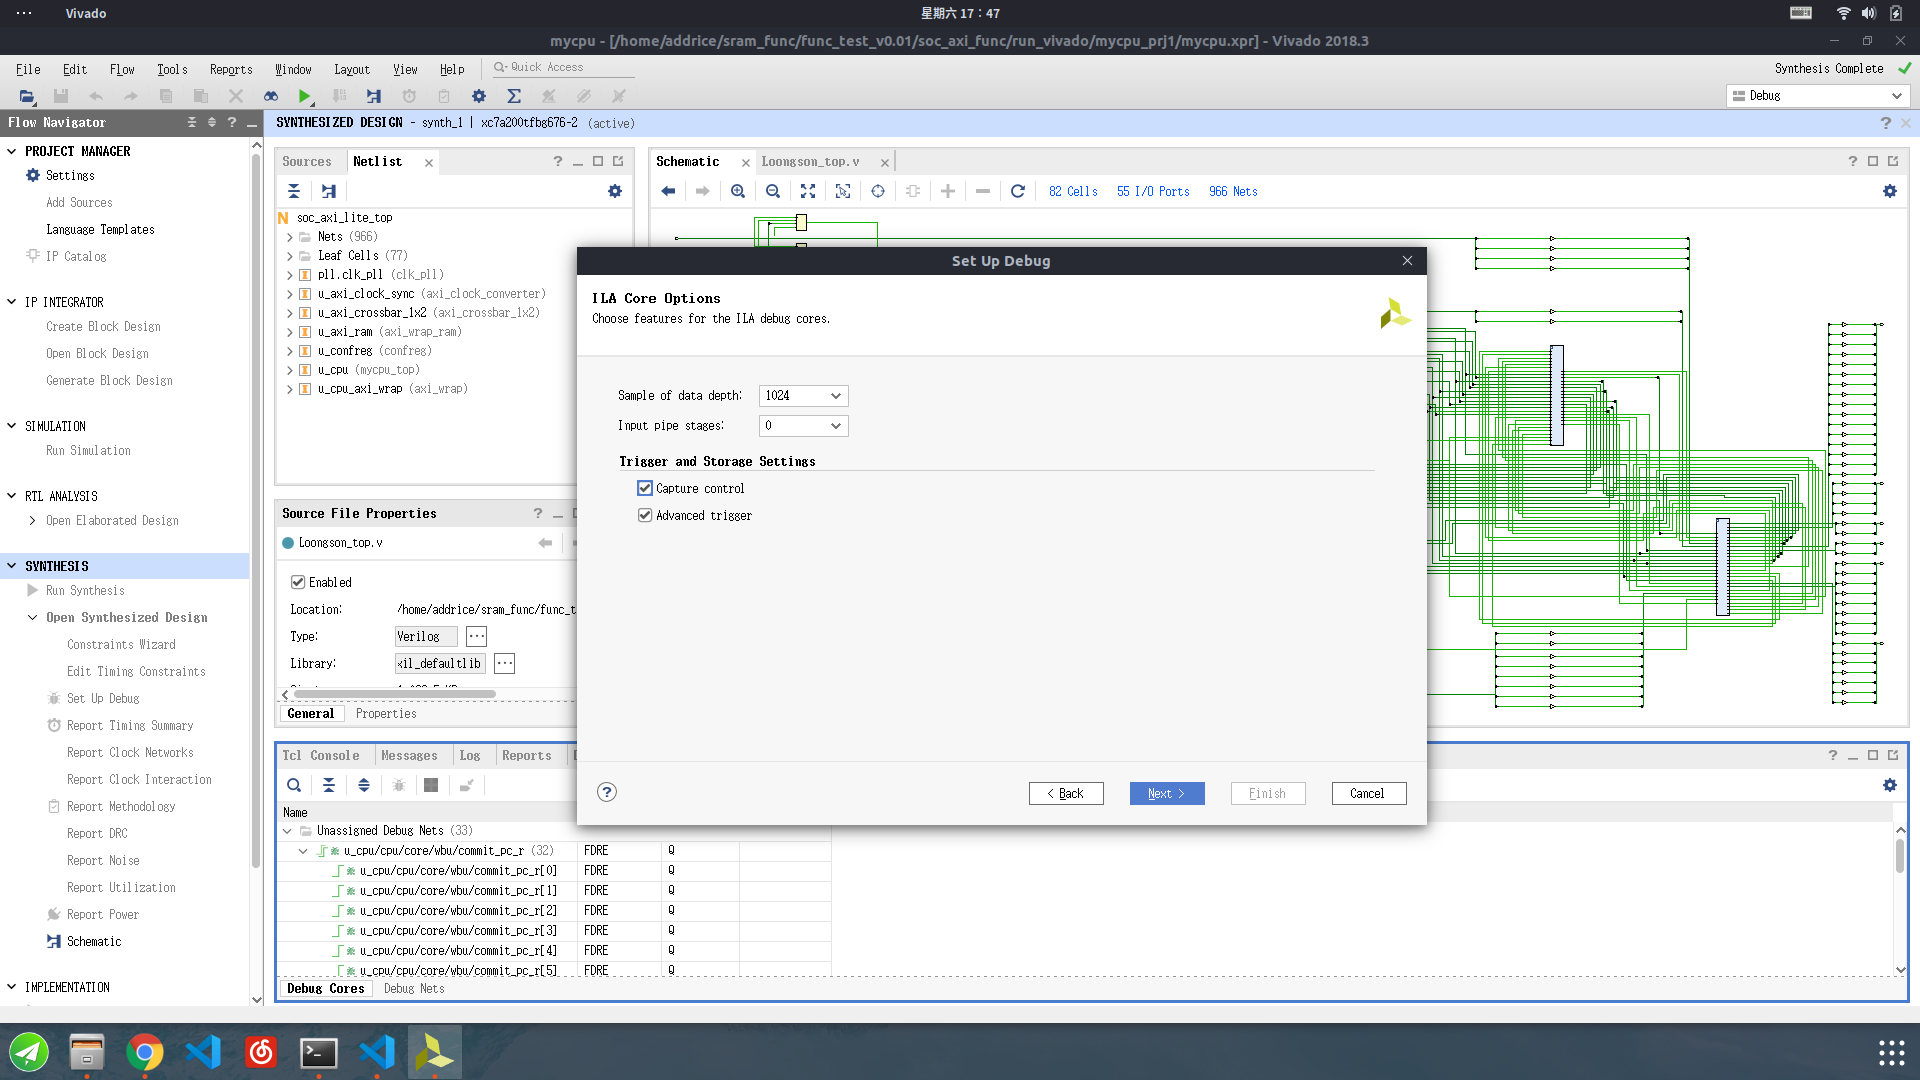
\includegraphics[width=\linewidth]{image/mark_debug_3.png}
\end{figure}
然后一路next完成。这一操作会修改我们的引脚文件,点击生成bitstream,save我们对综合文件的修改,如图所示
\begin{figure}[H]
\centering
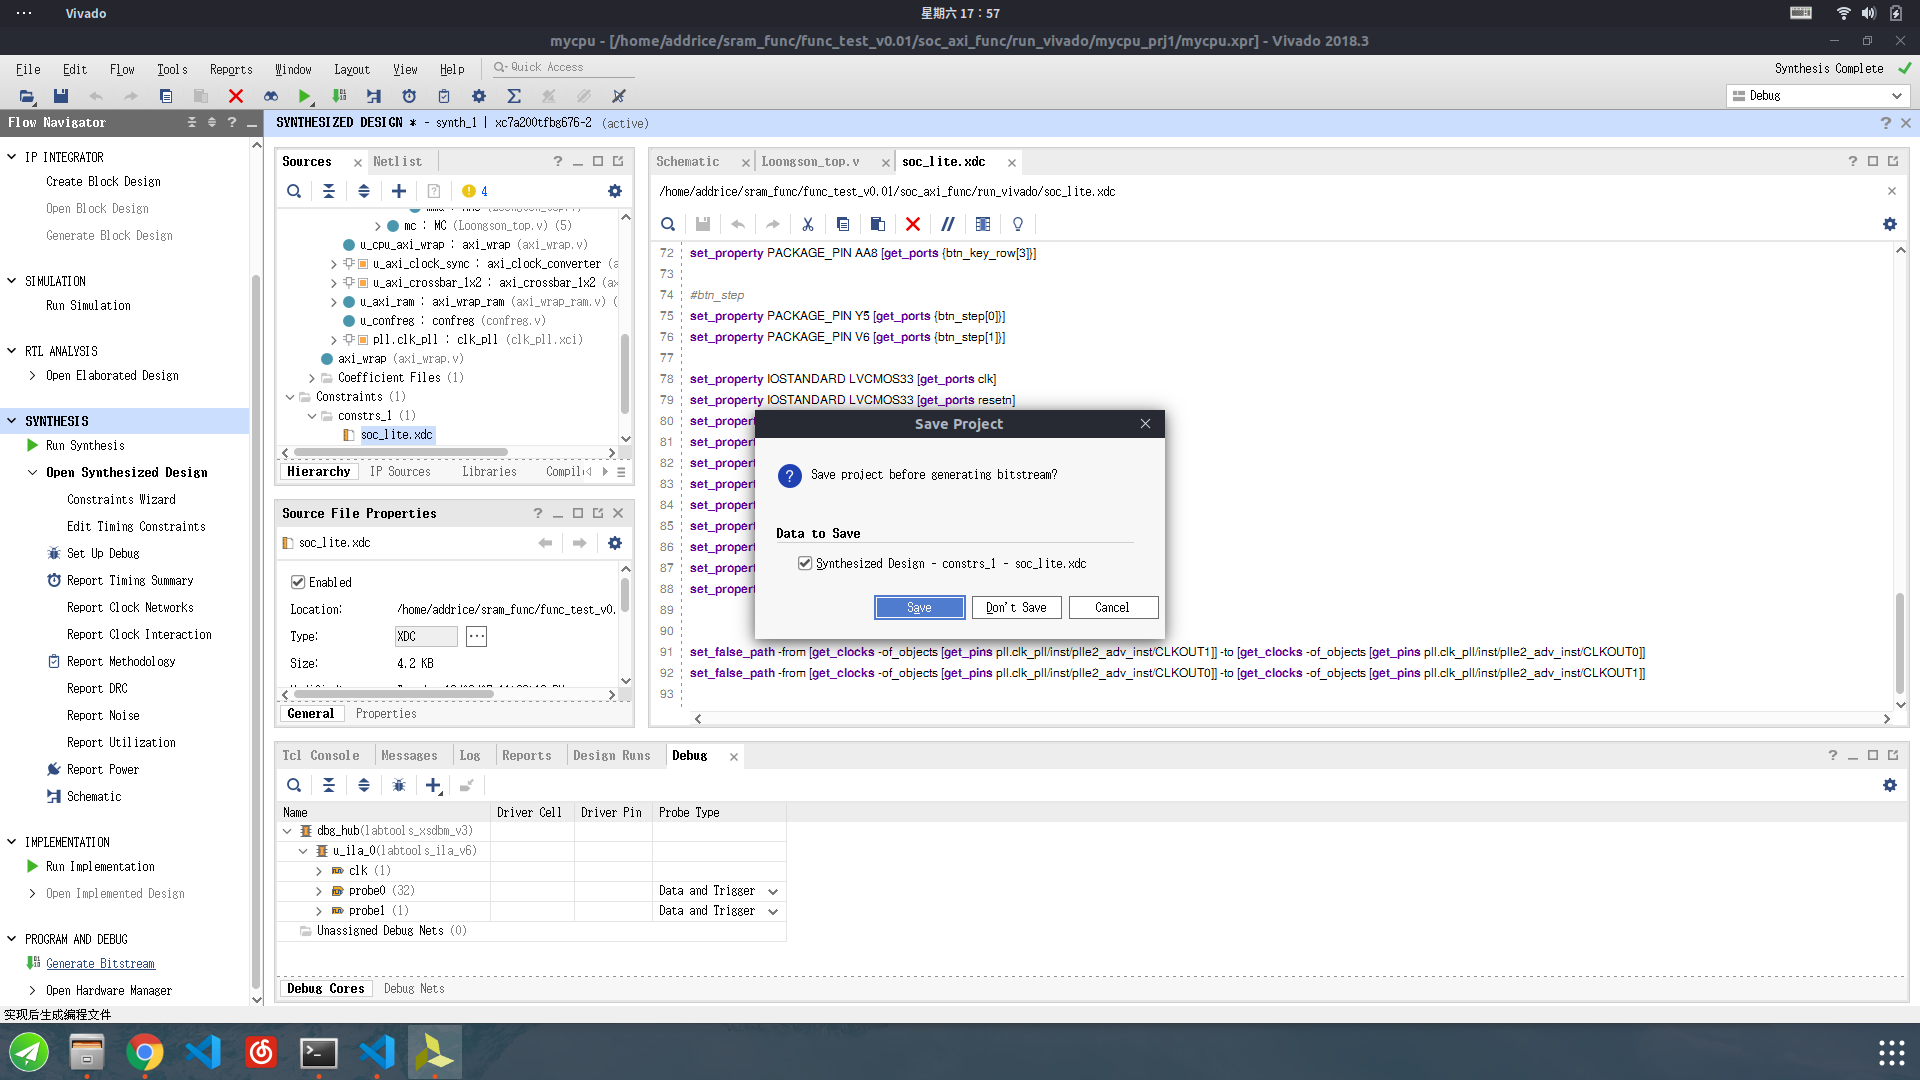
\includegraphics[width=\linewidth]{image/mark_debug_4.png}
\end{figure}
等待bitstream生成完毕上板即可。

\subsubsection{block design上使用system ila}

后来者待续

\section{MIPS相关}

\subsection{nju-mips简介}

\subsubsection{CPU Core}
\begin{itemize}
\item 单周期CPU
\item 多周期CPU(考虑信号的阻塞)
\item 一般流水线CPU(标准5段、score board)
\begin{itemize}
\item 长延迟指令(访存,乘除法)
\end{itemize}
\item 高级流水线CPU (分支预测器、ICache、DCache)
\begin{itemize}
\item CP0 (中断、异常)
\item L2 cache
\item TLB
\end{itemize}
\item 乱序流水线CPU(rename table、issue queue、ls queue、rob)
\item 乱序双发射CPU
\end{itemize}

\subsubsection{MIPS standard}
参见手册(\href{run:../manuals/MIPS_Vol1.pdf}{[1]}, \href{run:../manuals/MIPS_Vol2.pdf}{[2]}, \href{run:../manuals/MIPS_Vol3.pdf}{[3]})
\begin{itemize}
\item ALU: 算术运算指令(确定延迟)
  \begin{itemize}
  \item add, addu, addi, addiu, sub, subu, and, andi, clz, or, ori, xor, xori, nor, slt, sltu, slti, sltiu, sll, sllv, srl, srlv, sra, srav, lui, movn, movz
  \item 注意:clz有高效的递归,采用低效方案容易形成关键路径
  \end{itemize}
\item BRU: 分支跳转指令
  \begin{itemize}
  \item beq, bgtz, blez, bltz, bgez, bltzal, bgezal, bne, j, jal, jalr, jr
  \item 注意:所有的分支指令都有延迟槽,即分支后一条指令一定执行
  \end{itemize}
\item LSU: 访存指令(不定延迟)
  \begin{itemize}
  \item 对齐访存指令: lb, lbu, lh, lhu, lw, sb, sh, sw
  \item 不对齐访存指令: lwl, lwr, swl, swr
  \item 原子性读写指令: ll, sc
  \end{itemize}
\item MDU: 乘除法指令(长延迟)
  \begin{itemize}
  \item mul, mult, multu, div, divu, mfhi, mflo, mthi, mtlo
  \item 建议:hi和lo寄存器随通用寄存器一起进行转发,如果单独放在MDU里面,后续高级流水线的时候需要两套处理方案
  \end{itemize}
\item PRU: 特权指令(该单元又名CP0),重点看\href{../manuals/MIPS_Vol3.pdf}{[3]}
  \begin{itemize}
  \item syscall: 发起系统调用的指令
  \item eret: 系统调用执行完从内核态返回用户态的指令
  \item mfc0: cp0有自己的一套标准规定的寄存器,这条指令用于读cp0寄存器到一般寄存器
  \item mtc0: 用于将一般寄存器的值写入cp0
  \item tlbp: 用于查询一个虚拟地址的页表项是否存在
  \item tlbr: 用于读取一个页表项(cp0维护虚拟地址到物理地址的映射,形式有标准规定)
  \item tlbw: 用于写入一个页表项
  \item tlbwr: 由硬件随机淘汰一个旧页表项,并将新表项写入
  \item cache: 用于控制cache,包括将cache的一行写回,标记为无效等操作
  \item pref: 内存预取指令,用于加速,具体实现的时候可以什么都不做
  \item sync: 多核之间同步的指令,单核可以什么都不做
  \item break: 抛异常就行了
  \item tlt, tge, tltu, tgeu, tlti, teqi, tgei, tnei, tltiu, tgeiu, tne, teq: 自陷指令,条件满足的时候让cpu停住,不要抛异常了,直接在开发板上点个灯,正常执行是不会有这条指令的
  \end{itemize}
\item CP0: 0号协处理器
  \begin{itemize}
  \item 维护页目录,页目录缺失由操作系统回填,硬件抛异常就行了
  \item 维护cp0寄存器,以优先级排序:
    \begin{itemize}
    \item status, cause, epc (实现系统调用必须)
	\item badvaddr (实现异常必须,用于指示最后一个出错的访存地址)
	\item index, pagemask, context, entry\_lo0, entry\_lo1, entry\_hi (实现虚存必须)
	\item count, compare (实现时间中断必须)
	\item prid, config, config1 (运行u-boot和linux必需)
	\item base (可选,旧标准内没有,用于调整异常向量表的基址,缺省为0xbfc00000)
      \begin{itemize}
	  \item cpu启动时也是0xbfc00000,所以异常向量一般需要后期写入
      \end{itemize}
    \end{itemize}
  \end{itemize}
\item CP0寄存器的布局
  \begin{itemize}
  \item 寻址: (待续)
  \end{itemize}
\end{itemize}

\subsubsection{CPU uncore}

\begin{itemize}
\item \href{run:../manuals/AXI4.pdf}{[AXI4]}: 最常用的核外总线协议
  \begin{itemize}
  \item 几乎绝大多数硬件的IP核都会使用这个协议
  \item AXI4lite, 简化版的AXI4,但是不支持burst传输,一开始可以用这个
  \end{itemize}
\item Uartlite (用axi4-uartlite的IP核就行,无需自行实现)
  \begin{itemize}
  \item 最简单的串口协议
  \item 连接串口的简单[教程](docs/minicom.md)
  \end{itemize}
\item Emaclite (不需要深入理解、用就可以了)
  \begin{itemize}
  \item 最简单的网口协议
  \end{itemize}
\item VGA (用往届的就可以了)
  \begin{itemize}
  \item 数电课的VGA控制器包装成AXI4控制接口
  \end{itemize}
\item BlockRAM、RAM
  \begin{itemize}
  \item 片上资源,BlockRAM是读写均同步,适合用来做cache
  \item RAM,写同步,读异步,适合用来做register
  \end{itemize}
\end{itemize}

\subsubsection{CPU调试常用的工具链}
\begin{itemize}
\item Makefile \ref{Makefile}
  \begin{itemize}
  \item 用于将一键化各种功能
  \end{itemize}
\item tcl脚本
  \begin{itemize}
  \item vivado的自动化脚本,可以调用vivado的功能
  \item 如果需要一键创建vivado项目,这个是常用的工具
    \begin{itemize}
    \item vivado可以将当前项目导出到tcl脚本
    \end{itemize}
  \end{itemize}
\item block design
  \begin{itemize}
  \item 用图形界面来连接模块和IP核
  \end{itemize}
\item verilator \ref{verilator}
  \begin{itemize}
  \item verilog的模拟器,非常快,可以方便你们回归测试
  \item 到后期,用到IP核的时候,还需要用vivado的仿真工具
  \item 样例工程在`examples/1.Makefile-chisel-sample`中
  \end{itemize}
\item chisel
  \begin{itemize}
  \item 高级硬件描述语言
  \item 样例工程在`examples/1.Makefile-chisel-sample`中
  \end{itemize}
\item ILA
  \begin{itemize}
  \item 调试的终极大招,可以在板上电路中采样信号
  \end{itemize}
\end{itemize}

\subsection{CLZ的递归高效实现}
\subsubsection{函数版本}

\begin{lstlisting}
object CountLeadingZeros32 {
  def apply(in: UInt):UInt = {
    val out = Wire(Vec(5, Bool()))

    out(4) := in(31, 16) === 0.U(16.W)

    val val16 = Mux(out(4), in(15, 0), in(31, 16))
    out(3) := val16(15, 8) === 0.U(8.W)

    val val8  = Mux(out(3), val16(7, 0), val16(15, 8))
    out(2) := val8(7, 4) === 0.U(4.W)

    val val4  = Mux(out(2), val8(3, 0), val8(7, 4))
    out(1) := val4(3, 2) === 0.U(2.W)

    out(0) := Mux(out(1), ~val4(1), ~val4(3))

    Mux(in === 0.U, 32.U, out.asUInt)
  }
}
\end{lstlisting}

\subsubsection{模块版本(不建议使用)}

\begin{lstlisting}
class CountLeadingZeros32 extends Module {
  val io = IO(new Bundle {
	val in = Input(UInt(32.W))
	val out = Input(UInt(32.W))
  })

  val tmp = Wire(Vec(5, Bool()))

  tmp(4) := io.in(31, 16) === 0.U(16.W)

  val val16 = Mux(tmp(4), io.in(15, 0), io.in(31, 16))
  tmp(3) := val16(15, 8) === 0.U(8.W)

  val val8  = Mux(tmp(3), val16(7, 0), val16(15, 8))
  tmp(2) := val8(7, 4) === 0.U(4.W)

  val val4  = Mux(tmp(2), val8(3, 0), val8(7, 4))
  tmp(1) := val4(3, 2) === 0.U(2.W)

  tmp(0) := Mux(tmp(1), ~val4(1), ~val4(3))

  io.out := Mux(io.in === 0.U, 32.U, tmp.asUInt)
}
\end{lstlisting}

\section{相关项目说明}

\section{运行及移植linux}

\newpage

\nocite{*}
%\bibliographystyle{unsrt}
\bibliography{reference}

\end{document}
